\begin{frame}
  {Bildungssprache in der siebten Jahrgangsstufe}
  \pause
  Aufgabe: In eigenen Worten die Aufgabe wiedergeben\\
  (\citealt{GogolinLange2011}; s.\ \citealt{Feilke2012}).\\[0.5\baselineskip]
  \pause
  \centering
  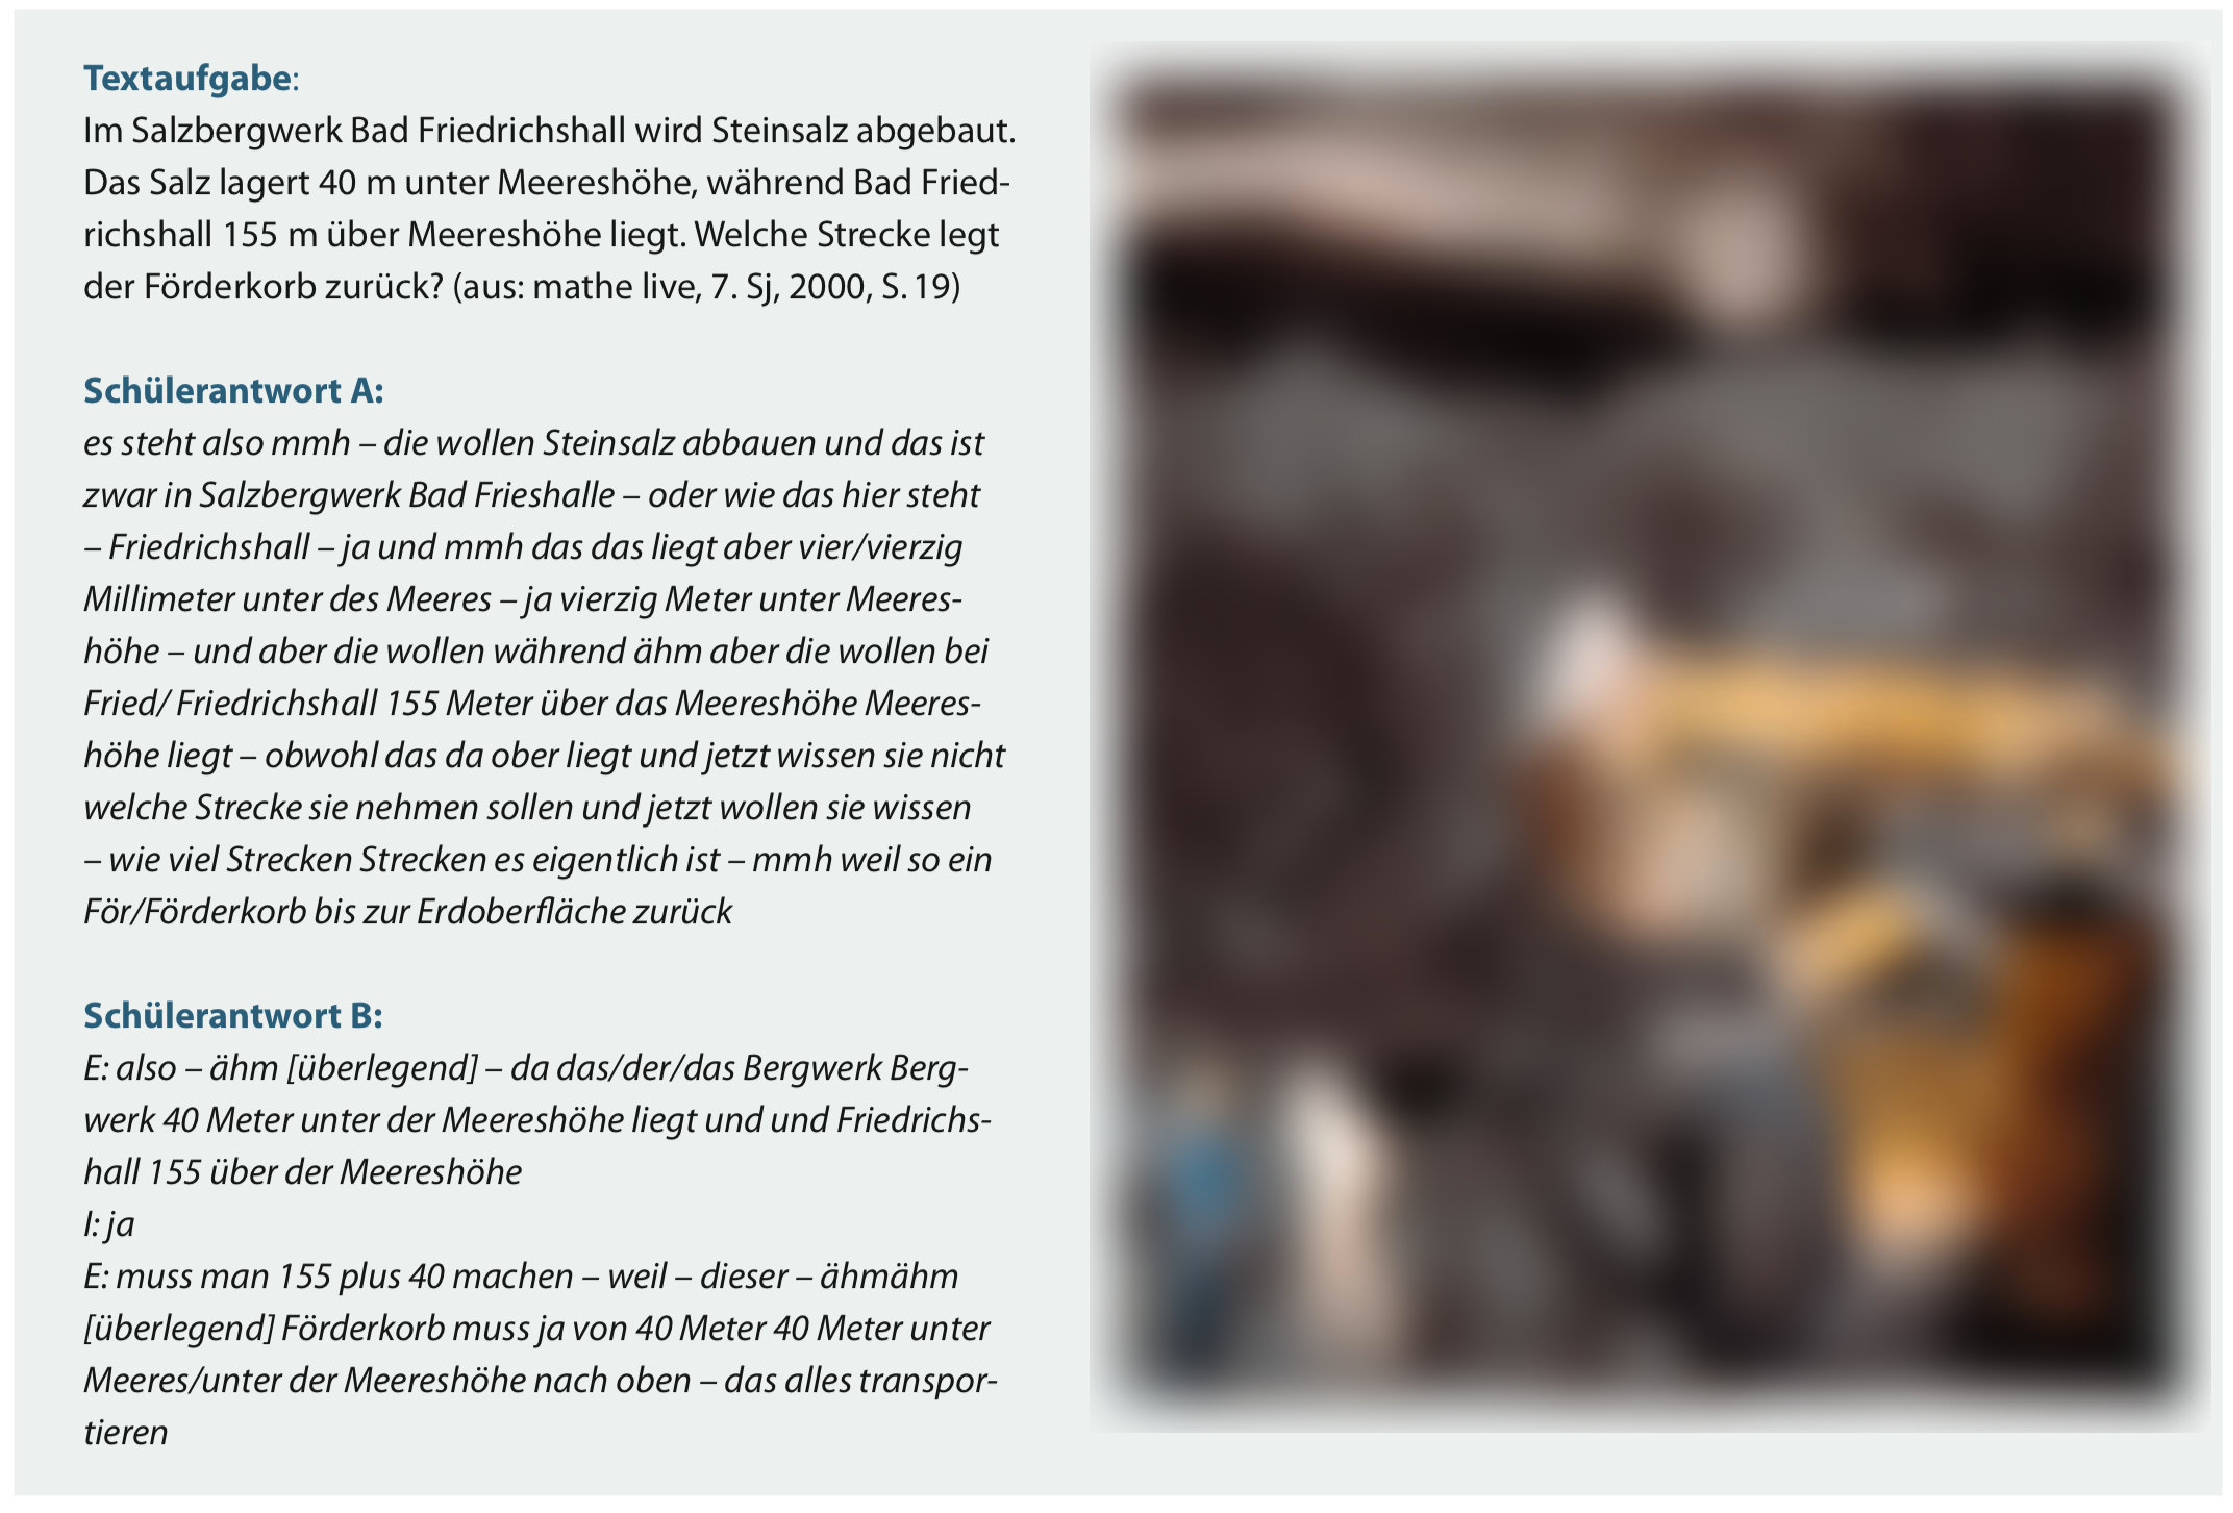
\includegraphics[height=0.68\textheight]{\GRAPHPATH/feilke_blur}
\end{frame}

\begin{frame}
  {Sprachbetrachtung und Literatur im Deutsch-Abitur I}
  \pause
  Sprachlich-grammatische Betrachtung zur Literatur in Abiturarbeiten\\
  \citep{Haecker2009}.\\[\baselineskip]
  \pause
  \centering
  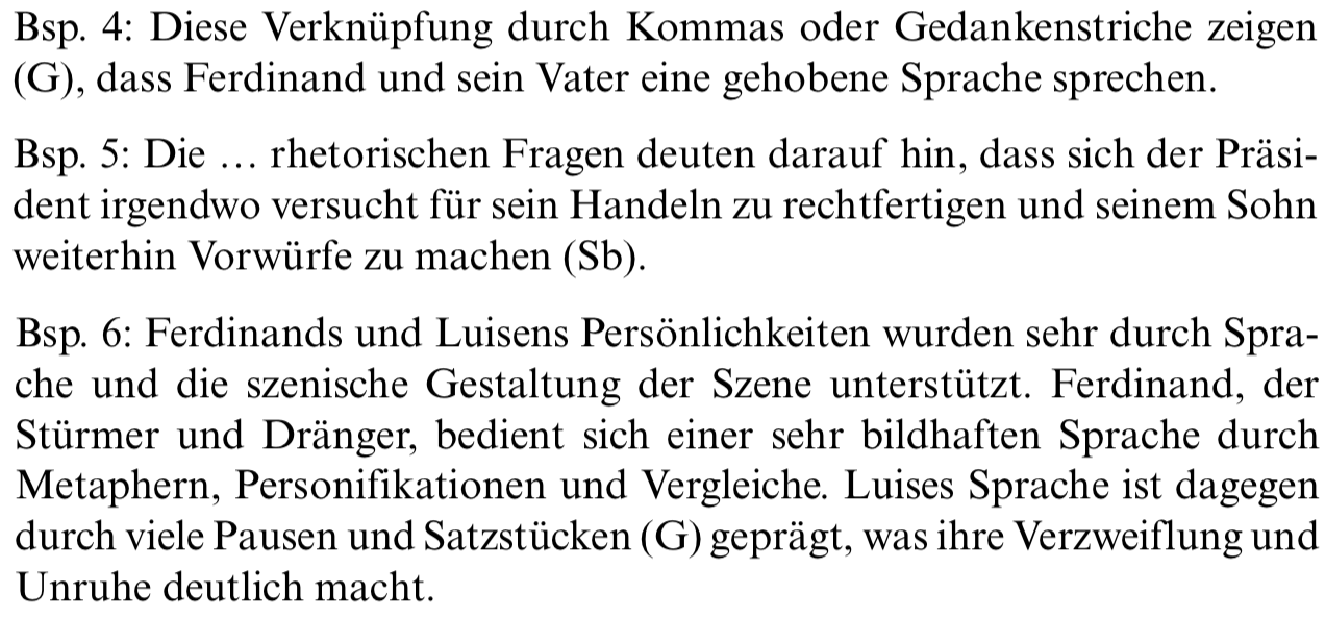
\includegraphics[height=0.5\textheight]{\GRAPHPATH/haecker1}
\end{frame}

\begin{frame}
  {Sprachbetrachtung und Literatur im Deutsch-Abitur II}
  Sprachlich-grammatische Betrachtung zur Literatur in Abiturarbeiten\\
  \citep{Haecker2009}.\\[\baselineskip]
  \centering
  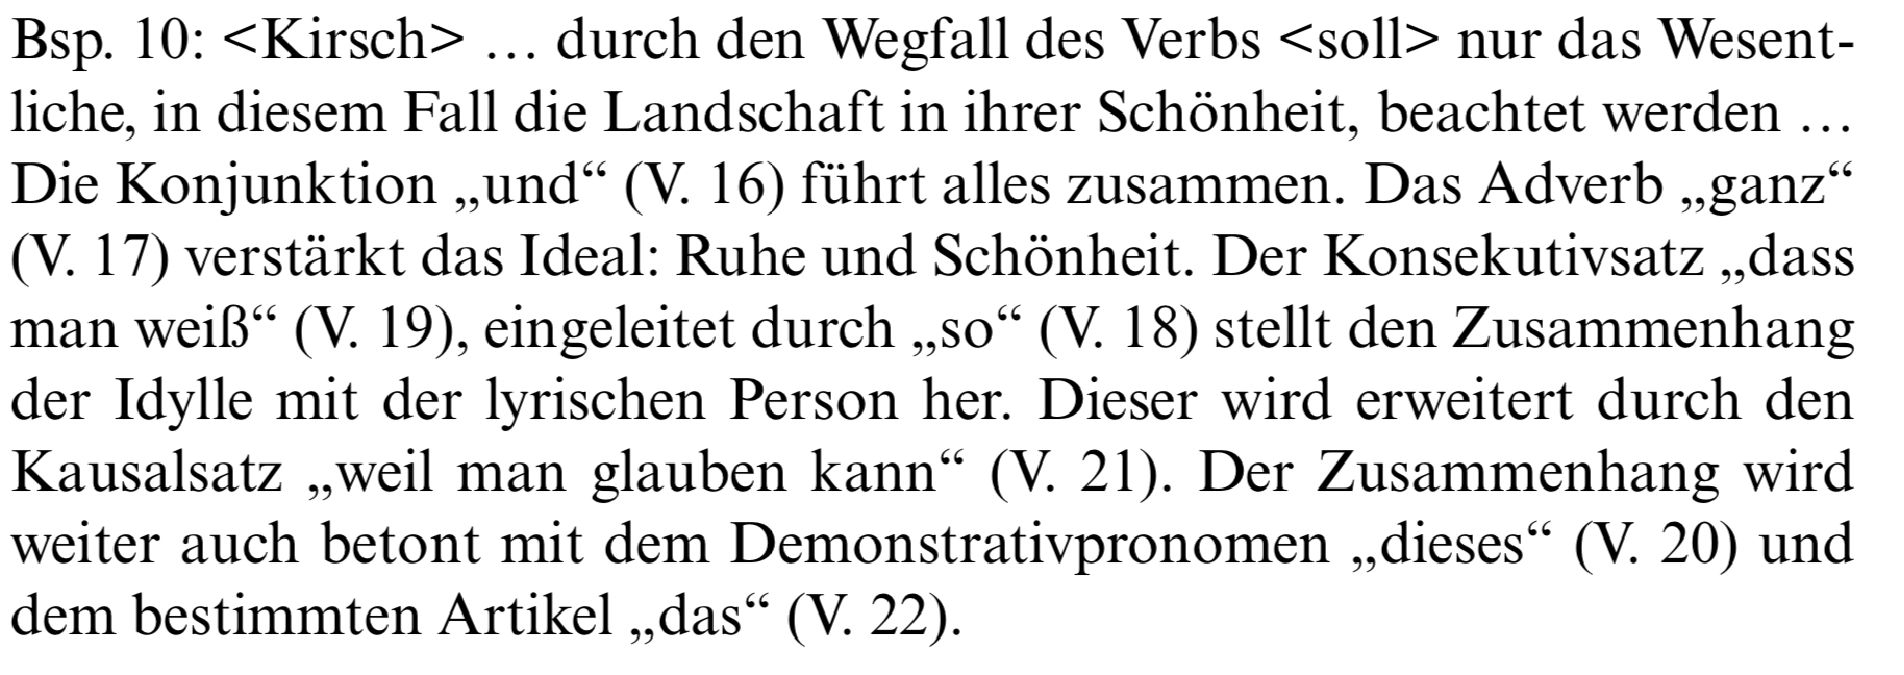
\includegraphics[height=0.4\textheight]{\GRAPHPATH/haecker2}
\end{frame}

\begin{frame}
  {Bildungssprache}
  \pause
  \alert{\textit{Der Deutschunterricht führt zu einem kompletten Umbau\\
  der Grammatik des Kindes.}} (nach \citealt{Bredel2013,Eisenberg2004})\\[\baselineskip]
  \pause
  \begin{itemize}[<+->]
    \item Anforderungen:
    \begin{itemize}[<+->]
      \item Darstellung komplexer Sachverhalte
      \item \dots und nicht-faktischer (z.\,B.\ hypothetischer) Sachverhalte
      \item Intensionalität
      \item Registerbewusstsein
    \end{itemize}
        \vspace{\baselineskip}
      \item Eigenschaften:
    \begin{itemize}[<+->]
      \item dekontextualisiert
      \item schriftorientiert
      \item normorientiert
    \end{itemize}
        \Halbzeile
      \item \alert{Das alles ist verknüpft mit spezifischen grammatischen Formen!}
  \end{itemize}
\end{frame}

\begin{frame}
  {Sprachbetrachtung}
  \pause
  \begin{itemize}[<+->]
    \item Bildungssprache $\Leftrightarrow$ Sprachbetrachtung
      \vspace{\baselineskip}
    \item Bewusstsein über richtige und angemessene Form
      \vspace{\baselineskip}
    \item explizite Sprachbetrachtung im Alltag:
      \begin{itemize}[<+->]
        \item Selbst- oder Fremdkorrektur
        \item Suche nach dem richtigen Ausdruck
        \item Orthographie optimieren
        \item Texte optimieren
        \item Begriffe definieren
        \item Grammatikalität beurteilen
      \end{itemize}
  \end{itemize}
\end{frame}

\begin{frame}
  {Ausgangsbasis: vorliterate Kinder und Sprachbetrachtung}
  \pause
  Klassische Studien nach \citet{Bredel2013}, s.\,a.\ \citet[57--58]{Schaefer2018}:\\
  \vspace{\baselineskip}
  \pause
  \begin{itemize}[<+->]
    \item \alert{bedeutungsbezogene} bzw.\ \alert{holistische} Betrachtung
    \item \textit{Welches Wort ist länger: Haus oder Streichholzschächtelchen?} --- \textit{Haus.}
    \item Assoziationen zu Substantiven wie \textit{Bett}: \alert{Ereignisse} \textit{schlafen gehen} usw.\\
      Erwachsene: \alert{Substantive} für andere Möbel usw.
    \item \textit{Warum heißt der Geburtstag  "`Geburtstag"'?} ---\\
      \textit{"`Weil es Geschenke und Kuchen gibt."'}
    \item \textit{Wieviele Wörter in "`Im alten Haus lebt eine junge Frau."'} --- \textit{Zwei.}
    \item \textit{Wieviele Wörter in "`Alex hat sieben Schwestern."'} --- \textit{Sieben.}
      \vspace{\baselineskip}
    \item Aber \alert{erfolgreich}: \textit{Benenne das letzte Wort des Satzes.}
    \item[$\Rightarrow$] Die mentale Grammatik basiert auf Wörtern,\\
      der sprachbetrachtende Zugriff allerdings noch nicht.
  \end{itemize}
\end{frame}

\begin{frame}
  {Schulunterricht}
  \begin{itemize}[<+->]
    \item \alert{systematisch}
      \begin{itemize}
        \item in knapper Zeit das Ganze im Blick
      \end{itemize}
      \vspace{\baselineskip}
    \item funktional im Sinn von \alert{Form-Funktion-Beziehung}
      \begin{itemize}
        \item Formen systematisieren
        \item erst dann auf Funktionen beziehen
      \end{itemize}
      \vspace{\baselineskip}
    \item \alert{induktiv}
      \begin{itemize}
        \item keine rein deduktive Anwendung vorgegebener Begriffe
        \item Erkenntnisprozesse über sprachliche Formen und Funktionen
        \item \alert{\textit{Grammatik machen}} (Eisenberg)
      \end{itemize}
  \end{itemize}
\end{frame}

\begin{frame}
  {Aufgaben von Lehrpersonen}
  \pause
  \alert{\textit{Lehrkräften wird die Sprache der Lernenden anvertraut.}} \citep{Eisenberg2004}\\[\baselineskip]
  \pause
  \begin{itemize}[<+->]
    \item Unterrichten der Schrift, Orthographie und Schreibung
    \item Unterweisung in Bildungssprache\slash Sprachbetrachtung
    \item Erkennen und \alert{Einordnen} von \alert{sprachlichen Defiziten}
    \item Erkennen von \alert{Interferenz mit Dialekt bzw.\ anderen Erstsprachen}
    \item \alert{Bewerten} von sprachlichen Leistungen
    \item \alert{Erklären} der Bewertung (auch gegenüber Eltern)
      \vspace{\baselineskip}
    \item[$\Rightarrow$] Anforderung: vertieftes Wissen über Sprache, vor allem Grammatik
    \item[$\Rightarrow$] Methode der sprachlichen Analyse über Faktenwissen hinaus
    \item[$\Rightarrow$] \rot{Die Grammatik für Studierende des Lehramts ist eine völlig andere\\
      als die, die sie später an Schulkinder und Jugendliche vermitteln!}
  \end{itemize}
\end{frame}


\begin{frame}
  {Wie war das?}
  Ich wiederhole zur Sicherheit nochmal\ldots\\
  \vspace{\baselineskip}
  \pause
  \begin{center}
    \Large\rot{Die Grammatik für Studierende des Lehramts\\
    ist eine völlig andere als die, die sie später \\
    an Schulkinder und Jugendliche vermitteln!}
  \end{center}
\end{frame}

\begin{frame}
  {"`Wozu brauchen wir das denn?"'}
  \pause
  \begin{itemize}[<+->]
    \item Diese Frage gilt hiermit als nachhaltig beantwortet.
    \item Linguistik und Fachdidaktik: keine praktische Anleitungen\\
      für erfolgreiche Schulstundenkonzepte
    \item Grundausbildung im \alert{Umgang mit Sprache} (Linguistik)\\
      und zum \alert{richtigen Handeln im Unterricht} (Fachdidaktik)
      \vspace{\baselineskip}
    \item Minimalforderung: \alert{Examinierte Lehrkräfte müssen\\
      die Aufgaben für die späteren Lernenden selber lösen und\\
      in den Gesamtkontext einordnen können.}
    \item \alert{Bis nächste Woche: Bitte schauen Sie sich den Fragebogen\\
      aus Schäfer \& Sayatz (2017) an (siehe Blackboard und Webseite).}
  \end{itemize}
\end{frame}

\section{Vorschau}

\begin{frame}
  {Phonetik: die Beschreibung der Aussprache}

  \begin{itemize}[<+->]
    \item Besprechung des Fragebogens sowie \citet{SchaeferSayatz2017a}
      \Zeile
    \item Medien der Sprachübermittlung
    \item Wie bilden wir Sprachlaute?
    \item Wo bilden wir Sprachlaute?
    \item deutsche Standardaussprache (Bundesrepublik)
    \item genaue Transkription von Sprachlauten
  \end{itemize}
  \pause
  \Halbzeile
  \begin{center}
    \rot{Lesen Sie bitte: Kapitel 4 \textit{Phonetik}}
  \end{center}

  \pause
  \pause
  \pause
  \pause
  \pause
\end{frame}
